% !TEX root = ./Vorlesungsmitschrift AGLA 2.tex  
\lecture{Fr 24.10. 10:15}{}
\file{Durchschnitt und Verbindung affiner Räume}
\section{Durchschnitt und Verbindung affiner Räume}
\begin{frage*}
    Sei \( X \) ein affiner Raum, \(    Y_1, Y_2 \) affine Unterräume von \( X \). Sind \( Y_1\cap Y_2, Y_1\cup Y_2 \) auch affine Unterräume von \( X \)?
    \begin{figure}[H]
        \centering
        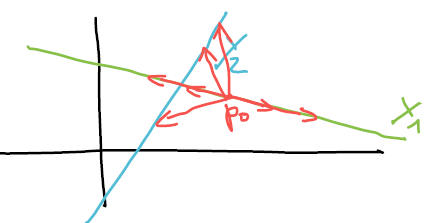
\includegraphics[width=0.5\linewidth]{figures/verbindung_affine_raeume}
        \caption*{\( X=\reals^2 \)}
        \label{fig:verbindung_affine_raeume}
    \end{figure}
\end{frage*}
\begin{lemma}\label{schnittraum:translationen}
    Sei \( X \) ein affiner Raum, \( Y_i \), \( i\in I \), eine Familie von affinen Unterräumen von \( X \).

    Dann ist \( Y\definedas \bigcap_{i\in I} Y_i \) ein affiner Unterraum von \( X \).

    Wenn \( Y\neq \emptyset \), dann gilt
    \begin{align*}
        T(Y)=\bigcap_{i\in I}T(Y_i).
    \end{align*}
\end{lemma}
\begin{proof}
    Falls \( Y=\emptyset \): \checkmark

    Wir nehmen also an \( Y\neq \emptyset \).
    Sei \( p_0\in Y \).
    Dann gilt:
    \begin{align*}
        T(Y)\begin{aligned}[t] 
            &=\Set{\underrelate{\textcolor{Goldenrod}\vertni}{\textcolor{Goldenrod}{T(X)}}{\vv{p_0 q}},q\in \bigcap_{i\in I}Y_i}\\
            &=\bigcap_{i\in I}\textcolor{LimeGreen}{\underbrace{\Set{\vv{p_0 q}, q\in Y_i}}_{=T(Y_i)}}\\
            &=\bigcap_{i\in I}T(\explain[big]{\text{Untervektorräume von \( T(X) \)}}{Y_i}).
        \end{aligned}
    \end{align*}
    Also ist \( T(Y) \) ein Untervektorraum von \( T(X) \) und \( T(Y)=\bigcap_{i\in I}T(Y_i) \).
\end{proof}
\begin{bemerkung*}
    In obiger Notation ist \( \bigcup_{i\in I}Y_i \) im Allgemeinen kein affiner Unterraum von \( X \).
\end{bemerkung*}
\begin{frage*}
    Finde den \enquote{kleinsten} affinen Unterraum von \( X \), der \( \bigcup_{i\in I}Y_i \) enthält! (\zb \( X\supseteq \bigcup_{i\in I} Y_i\), aber \( X \) ist im Allgemeinen nicht \enquote{minimal}).
\end{frage*}
\begin{definition*}
    Sei \( X \) ein affiner Raum, \( Y_i \), \( i\in I \) affine Unterräume von \( X \). Wir nennen
    \begin{align*}
        \bigcap_{\mathclap{\substack{Y\subseteq X \text{ aff.\ Unterraum}\\
         \bigcup_{i\in I}Y_i\subseteq Y}}}Y
    \end{align*}
    den \emph{Verbindungsraum} der affinen Unterräume \( Y_i \), \( i\in I \). Schreibe \( \bigvee_{i\in I}Y_i \).
\end{definition*}
\begin{beispiel*}
    \begin{figure}[H]
        \centering
        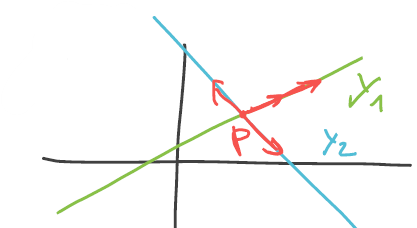
\includegraphics[width=0.5\linewidth]{figures/verbindungsraum_zwei_geraden}
        \caption*{\( X=\reals^2 \), \( Y_1\vee Y_2=X \), \textcolor{OrangeRed}{\( Y=Y_1\vee Y_2 \), \( T(Y)=T(Y_1)+T(Y_2) \)}.}
        \label{fig:verbindungsraum_zwei_geraden}
    \end{figure}
    
\end{beispiel*}

\begin{frage*}
    Wie kann man im Allgemeinen \( T(Y_1\vee Y_2) \) aus \( T(Y_1),T(Y_2) \) bestimmen?
\end{frage*}
\begin{lemma}\label{verbindungsraum:translationen}
    Sei \( X \) ein affiner Raum, \( Y_1,Y_2\neq\emptyset \) affine Unterräume von \( X \).
    \begin{eigenschaftenenumerate}
        \item \label{verbindungsraum:translationen:schnitt_nicht_leer}Sei \( Y_1\cap Y_2\neq \emptyset \).
        Dann gilt
        \begin{align*}
            T(Y_1\vee Y_2)=T(Y_1)+T(Y_2).
        \end{align*}
        
        \item \label{verbindungsraum:translationen:schnitt_leer}Sei \( Y_1\cap Y_2=\emptyset \), \( p_1\in Y_1, p_2\in Y_2\) und \( Y=p_1\vee p_2 \).
        
        Dann gilt:
        \begin{align*}
            T(Y_1\vee Y_2)=(T(Y_1)+T(Y_2))\oplus T(Y).
        \end{align*}
    \end{eigenschaftenenumerate}
\end{lemma}
\begin{proof}
    \begin{proofdescription}
        
        \item[\ref{verbindungsraum:translationen:schnitt_nicht_leer}]
        \begin{figure}[H]
            \centering
            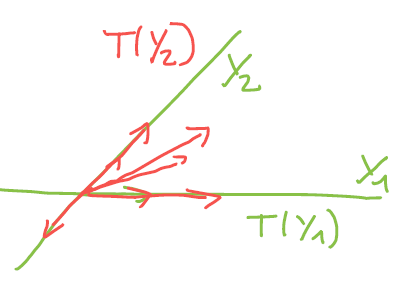
\includegraphics[width=0.5\linewidth]{figures/verbindungsraum_translationen_schnitt_nicht_leer}
            \label{fig:verbindungsraum_translationen_schnitt_nicht_leer}
        \end{figure}
         Sei \( p\in Y_1\cap Y_2 \). Dann gilt
         \begin{align*}
             T(Y_1)\cup T(Y_2)\begin{aligned}[t] 
                &=\Set{\vv{pq}|q\in Y_1\cup Y_2}\\
                &\subseteq T(Y_1\vee Y_2),
             \end{aligned}
         \end{align*}
         also \( T(Y_1)+T(Y_2)\subseteq T(Y_1\vee Y_2) \).

         Sei \( Y=\Set{\tau_t(p)|t\in T(Y_1)+T(Y_2)} \).
         Dann ist \( Y \) affiner Unterraum von \( X \) mit \( Y_1\cup Y_2\subseteq Y \), also \( Y_1\vee Y_2\subset Y \), also \( Y_1\vee Y_2\subseteq Y \). Also gilt
         \begin{align*}
             T(Y_1\vee Y_2)\subseteq T(Y)=T(Y_1)+T(Y_2).
         \end{align*}
         
         Also \( T(Y_1\vee Y_2)=T(Y_1)+T(Y_2) \).
         
         \item[\ref{verbindungsraum:translationen:schnitt_leer}]
         \( Y_1\cap Y_2=\emptyset \), \( p_1\in Y_1 \), \( p_2\in Y_2 \), \( Y=p_1\vee p_2 \).
         \begin{figure}[H]
             \centering
             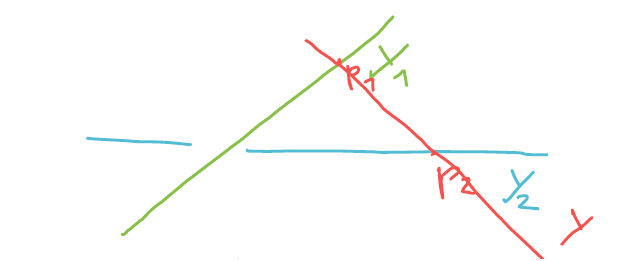
\includegraphics[width=0.5\linewidth]{figures/verbindungsraum_translationen_schnitt_leer}
             \label{fig:verbindungsraum_translationen_schnitt_leer}
         \end{figure}
         Schreibe \( Y_1\vee Y_2=Y_1\vee Y\vee Y_2 \) (verwende dazu \( Y\subseteq Y_1\vee Y_2 \)).
         Verwende \ref{verbindungsraum:translationen:schnitt_nicht_leer} und leite ab, dass gilt:
         \begin{align*}
             T(Y_1\vee Y \vee Y_2)\begin{aligned}[t] 
                 &=T(Y_1)+T(Y\vee Y_2)\\
                 &=T(Y_1)+T(Y)+T(Y_2)\\
                 &=(T(Y_1)+T(Y_2))\needed{\oplus} T(Y).
             \end{aligned}
         \end{align*}
         Es gilt 
         \begin{align*}
             T(Y)=\Set{\lambda\vv{p_1 p_2}| \lambda\in K}.
         \end{align*}
         Wir wollen zeigen
         \begin{align*}
             (T(Y_1)+T(Y_2))\cap T(Y)=\zeroset.
         \end{align*}
         Es genügt zu zeigen
         \begin{align*}
             \vv{p_1 p_2}\notin T(Y_1)+T(Y_2).
         \end{align*}
         Gegenannahme:
         \begin{align*}
             \vv{p_1 p_2}=\underrelate{\vertni}{T(Y_1)}{\vv{p_1 y_1}}+\underrelate{\vertni}{T(Y_2)}{\vv{q_2 p_2}}
         \end{align*}
         mit \( q_1\in Y_1 \), \( q_2\in Y_2 \).
         \begin{figure}[H]
             \centering
             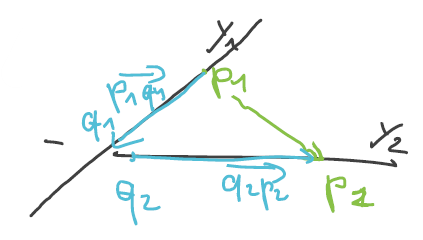
\includegraphics[width=0.5\linewidth]{figures/verbindungsraum_translationen_schnitt_leer_verbindungslinie_nicht_in_translationen}
             \label{fig:verbindungsraum_translationen_schnitt_leer_verbindungslinie_nicht_in_translationen}
         \end{figure}
         Dann gilt
         \begin{align*}
             \vv{q_1 q_2}=\vv{q_1 p_1}+\vv{p_1 p_2}+\vv{p_2 q_2}=0,
         \end{align*}
         also \( q_1=q_2 \) und \( Y_1\cap Y_2\neq \emptyset \) \contra.
    \end{proofdescription}
\end{proof}
Als nächstes: \( \affindim{Y_1\vee Y_2} \) ist durch \( \dim-{K}{T(Y_1\vee Y_2)} \) gegeben, also sollten wir aus \thref{verbindungsraum:translationen} für \( Y_1\vee Y_2 \) ableiten können.
\begin{lemma}\label{verbindungsraum:dimension}
    Sei \( X \) ein affiner Raum, \( Y_1, Y_2\neq \emptyset \) affine Unterräume von \( X \).
    \begin{eigenschaftenenumerate}
        \item\label{verbindungsraum:dimension:schnitt_nicht_leer} Sei \( Y_1\cap Y_2\neq \emptyset \).
         Dann gilt \( \dim(Y_1\vee Y_2)=\dim(Y_1)+\dim(Y_2)-\dim(Y_1\cap Y_2) \).
        \item\label{verbindungsraum:dimension:schnitt_leer} Sei \( Y_1\cap Y_2=\emptyset \).
        Dann gilt
        \begin{align*}
            \dim(Y_1\vee Y_2)=\dim(Y_1)+\dim(Y_2)-\dim(T(Y_1)\cap T(Y_2))+1.
        \end{align*}
    \end{eigenschaftenenumerate}
    
\end{lemma}
\begin{proof}
    \begin{proofdescription}
        
        \item[\ref{verbindungsraum:dimension:schnitt_nicht_leer}] Aus \thref{verbindungsraum:translationen} folgt
        \begin{align*}
            T(Y_1\vee Y_2)=T(Y_1)+T(Y_2),
        \end{align*}
        aus der Dimensionsformel für Untervektorräume folgt
        \begin{equation*}
            \affindim{Y_1\vee Y_2}\begin{aligned}[t] 
                &=\dim-{}{T(Y_1\vee Y_2)}\\
                &=\affindim{Y_1}+\dim-{}{T(Y_2)}-\dim{}{T(Y_1)\cap T(Y_2)}\\
                &\explain{\text{\thref{schnittraum:translationen}}}{=}\dim-{}{T(Y_1)}+\dim-{}{T(Y_2)}-\dim-{}{T(Y_1\cap Y_2)}\\
                &=\affindim-{Y_1}+\affindim-{Y_2}-\affindim-{Y_1\cap Y_2}.
            \end{aligned}
        \end{equation*}
        
        \item[\ref{verbindungsraum:dimension:schnitt_leer}] \( Y_1\cap Y_2 \), \( p_1\in Y_1 \), \( p_2\in Y_2 \), \( Y=p_1\vee p_2 \).
        
        Dann ist
        \begin{align*}
            \affindim-{Y}=\dim-{}{T(Y)}=1.
        \end{align*}
        Wir erhalten
        \begin{align*}
            \affindim{Y_1\vee Y_2}\begin{aligned}[t] 
                % &=\dim-{}{T(Y_1\vee Y_2)}\\
                % &\explain{\text{\thref{verbindungsraum:translationen}}}{=}\affindim{(T(Y_1)+T(Y_2))\oplus T(Y)}\\
                % &=\dim{}{T(Y_1)+T(Y_2)}+\equalto{1}\dim-{}{T(Y)}\\
                % &=\dim-{}{T(Y_1)}+\dim-{}{T(Y_2)}- \dim-{}{T(Y_1)\cap T(Y_2)}+1\\
                &=\affindim-{Y_1}+\affindim-{Y_2} -\dim{}{T(Y_1)\cap T(Y_2)}+1
            \end{aligned}
        \end{align*}
    \end{proofdescription}
\end{proof}
\begin{beispiel*}[\( X=\reals^3 \)]
    \begin{figure}[H]
        \centering
        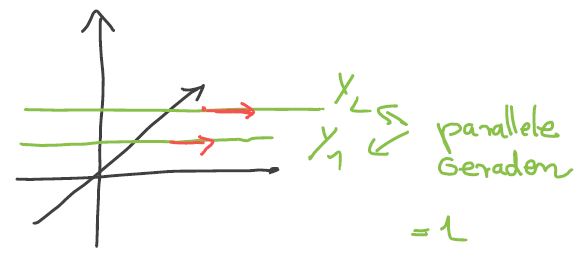
\includegraphics[width=0.5\linewidth]{figures/verbindungsraum_parallele_geraden}
        \label{fig:verbindungsraum_parallele_geraden}
    \end{figure}
    \begin{align*}
        \affindim{Y_1\vee Y_2}=1+1-\underbrace{\dim{}{T(Y_1)\cap T(Y_2)}}_{=1}+1=2
    \end{align*}
    \begin{figure}[H]
        \centering
        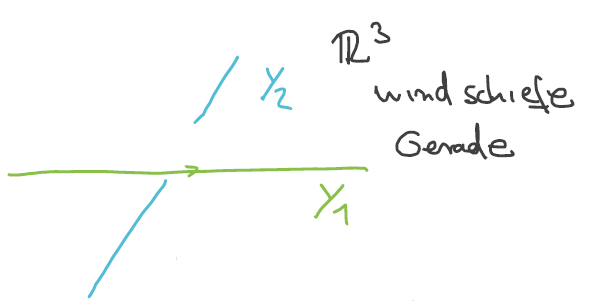
\includegraphics[width=0.6\linewidth]{figures/verbindungsraum_windschiefe_geraden}
        \label{fig:verbindungsraum_windschiefe_geraden}
    \end{figure}
    \begin{align*}
        \affindim{Y_1\vee Y_2}=1+1-0+1=3
    \end{align*}
    und \( Y_1\vee Y_2=X \).
    
\end{beispiel*}
\file{Parallelprojektionen}
\section{Parallelprojektionen}
\label{parallelprojektionen}
\begin{wiederholung*}[Projektionen aus der \aglacourse{1}]
    \begin{beispiel*}
        \begin{figure}[H]
            \centering
            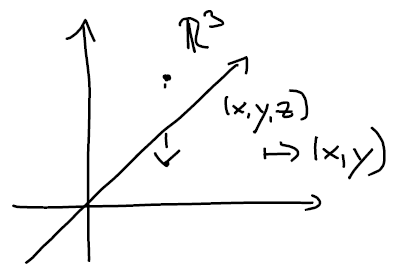
\includegraphics[width=0.5\linewidth]{figures/r_3_projektion}
            \label{fig:r_3_projektion}
        \end{figure}
        
    \end{beispiel*}
    Sei \( V \) ein \( K \)-Vektorraum, \( W, W_1\subset V \) \( K \)-Untervektorräume mit \( V=W\oplus W_1 \).
    Schreibe \( v\in V \) in der Form \( v=w+w_1 \) und mit \( w\in W \), \( w_1\in W_1 \). Definiere
    \begin{align*}
        P_W\maps \begin{aligned}[t] 
            V&\to W_1\\
            \equalto{w+w_1}{v}&\mapsto w_1.
        \end{aligned}
    \end{align*}
    Ein paar Eigenschaften von \( P_W \):
    \begin{itemize}
        \item \( P_W\maps V \to W_1 \) ist eine lineare Abbildung,
        \item \( \Ker-{P_W}=W \),
        \item \( \evaluateat{P_W}{W_1}=\Id_{W_1} \).
    \end{itemize}
    Als Nächstes:
    Wir schränken \( P_W \) ein auf einen Untervektorraum \( W_0 \) von \( V \).
    \begin{figure}[H]
        \centering
        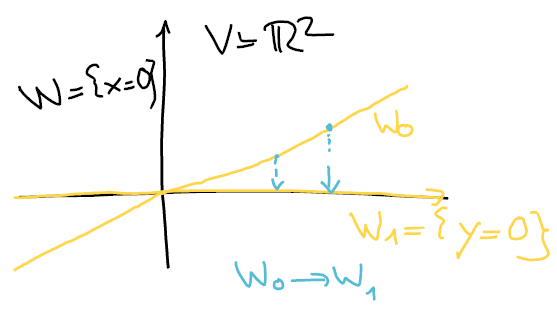
\includegraphics[width=0.5\linewidth]{figures/projektion_einschraenkung_auf_w_0}
        \label{fig:projektion_einschraenkung_auf_w_0}
    \end{figure}
    \begin{lemma}\label{projektion_isomorph}
        Sei \( V \) ein \( K \)-Vektorraum, \( W,W_0, W_1\subseteq V \) Untervektorräume mit \( V=W\oplus W_0=W\oplus W_1 \).

        Dann ist \( \evaluateat{P_W}{W_0}\maps W_0\to W_1 \) ein Isomorphismus (Notation wie oben).
    \end{lemma}
    \begin{proof}
        Es gilt \( \affindim-{W_0}=\affindim-{W_1} \) und es genügt zu zeigen, dass \( \evaluateat{P_W}{W_0} \) injektiv ist.

        Sei \( \evaluateat{P_W}{w_0}=w_1 \) für \( w_0\in W_0 \), \( w_1\in W_1 \). Dann ist \( w_0=w+w_1 \) mit \( w\in W \), \( w_1\in W_1 \), also
        \begin{align*}
            w_1=\underrelate{\textcolor{LimeGreen}{\vertni}}{\textcolor{LimeGreen}{W_0}}{w_0}-\underrelate{\textcolor{LimeGreen}{\vertni}}{\textcolor{LimeGreen}{W}}{w}\in W_0\oplus W,
        \end{align*}
        und diese Zerlegung ist eindeutig.
        
    \end{proof}
    
\end{wiederholung*}
\subsection*{Parallelprojektionen für affine Räume}
Sei \( X \) ein affiner Raum (über einem Körper \( K \)), \( Y_1\subseteq X \) ein affiner Unterraum
\begin{beispiel*}
    \begin{figure}[H]
        \centering
        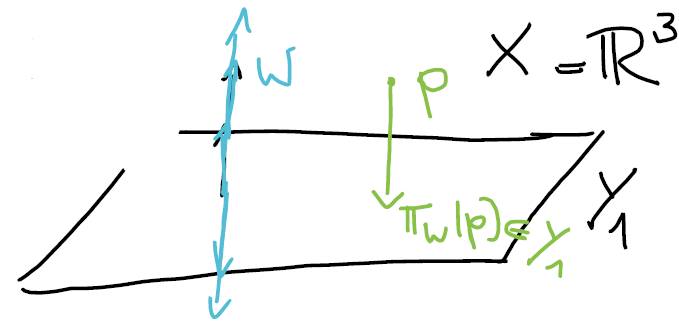
\includegraphics[width=0.5\linewidth]{figures/affine_parallelprojektion_r_3}
        \label{fig:affine_parallelprojektion_r_3}
    \end{figure}
    
\end{beispiel*}
Sei \( W\subseteq T(X) \) ein Untervektorraum mit \( T(X)=T(Y_1)\oplus W \).
\begin{ziel*}
    Definiere eine Projektionsabbildung
    \begin{align*}
        \pi_W\maps X\to Y_1
    \end{align*}
    \enquote{längs \( W \)}.
\end{ziel*}
Für \( p\in X \) definiere
\begin{align*}
    W(p)\definedas\Set{x\in X| \vv{px}\in W}
\end{align*}
\begin{lemma}
    Notation wie oben.
    Für \( p\in X \) gilt
    \begin{align*}
        \anzahl{Y_1\cap W(p)}=1.
    \end{align*}
\end{lemma}
\begin{proof}
    Wir berechnen
    \begin{align*}
        \affindim-{Y_1\cap W(p)}.
    \end{align*}
    Sei \( x=\affindim-{X} \), verwende \thref{verbindungsraum:dimension}~\ref{verbindungsraum:dimension:schnitt_leer}.
    Falls \( Y_1\cap W(p)=\emptyset \), dann
    \begin{align*}
        \affindim-{Y_1\vee W(p)}\begin{aligned}[t] 
            &=\affindim-{Y_1}+\affindim-{W(p)}-\affindim{\underbrace{T(Y_1)\cap W}_{\textcolor{LimeGreen}{=\zeroset}}}+1\\
            &=\dim-{}{T(Y_1)}+\affindim-{W}+1
        \end{aligned}
    \end{align*}
    \contra zu \( Y_1\vee W(p)\subseteq X \), also ist \( Y_1\cap W(p)\neq \zeroset \), und nach \thref{verbindungsraum:dimension}~\ref{verbindungsraum:dimension:schnitt_nicht_leer} gilt Folgendes:
    \begin{align*}
        \equalto{n}{\underbrace{\affindim{Y_1\vee W(p)}}}\begin{aligned}[t] 
            &=\affindim-{Y_1}+\affindim-{W(p)}-\affindim{Y_1\cap W(p)}\\
            &=n-\affindim{Y_1\cap W(p)}
        \end{aligned}
    \end{align*}
    und nach \thref{schnittraum:translationen}
    \begin{align*}
        \affindim-{Y_1\vee W(p)}\begin{aligned}[t] 
            &=\dim{}{T(Y_1)+W}\\
            &=n,
        \end{aligned}
    \end{align*}
    also \( \affindim{Y_1\cap W(p)}=0 \).
    
\end{proof}
Wir definieren die Projektion längs \( W \)
\begin{align*}
    \pi_W\maps \underrelate{\subseteq}{Y_0}{X}\to Y_1,\logicspace p\mapsto W(p)\cap Y_1.
\end{align*}
\begin{satz}
    Sei \( X \) ein affiner Raum, \( Y_1,Y_0\subseteq X \) affine Unterräume, \( W\subseteq T(X) \) ein Untervektorraum mit 
    \begin{align*}
        T(X)=W\oplus T(Y_0)=W\oplus T(Y_1).
    \end{align*}
    Dann ist \( \pi_W\maps X\to Y_1 \) eine surjektive affine Abbildung und \( \evaluateat{\pi_w}{Y_0}\maps Y_0\to Y_1 \) eine Affinität.
\end{satz}
\begin{proof}
    Seien \( p,q\in X \).
    \begin{figure}[H]
        \centering
        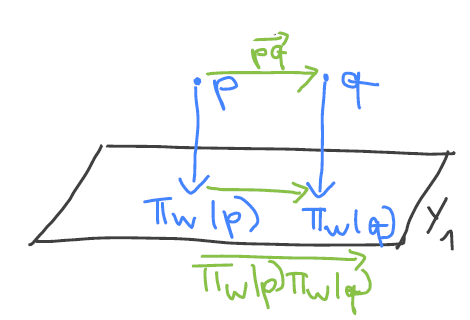
\includegraphics[width=0.5\linewidth]{figures/affine_projektion_ist_affin}
        \label{fig:affine_projektion_ist_affin}
    \end{figure}
    Dann gilt
    \begin{align*}
        \vv{pq}\begin{aligned}[t] 
            &=\vv{p\pi_W(p)}+\vv{\pi_W(p)\pi_W(q)}+\vv{\pi_W(q)q}+\vv{\pi_W(q)q}\\
            &=\underbrace{\vv{p\pi_W(p)}+\vv{\pi_W(q)q}}_{\textcolor{Cyan}{\in W}}+\underbrace{\vv{\pi_W(p)\pi_W(q)}}_{\textcolor{Cyan}{\in T(Y_1)}},
        \end{aligned}
    \end{align*}
    also \( \vv{\pi_W(p)\pi_W(q)}=P_W(\vv{pq}) \).

    \( P_W \) ist surjektiv, also ist \( \pi_W \) eine surjektive affine Abbildung.

    Der zweite Teil folgt aus \thref{projektion_isomorph}.
\end{proof}